% !TeX root = main.tex
% !TeX spellcheck = en-US
% !TeX encoding = utf8


\chapter{Results and Evaluation}
\label{chap:results}

All experiments and analyses were performed as previously explained in \cref{chap:testing,chap:analysis}. 

\section{Part I - Choosing the Optimization Algorithm}
\label{chap:part1}
The results of the first experimentation part are very insightful and allow for a sound analysis of the most appropriate optimization algorithm to tune the parameters of the \gls{hsppbo} algorithm. Note that an evaluation of the quality of the solution itself and of the performance of the \gls{hsppbo} algorithm is not discussed in this first part. The solution quality is only used to compare the optimization methods. 

\begin{figure}[h]
	\centering
	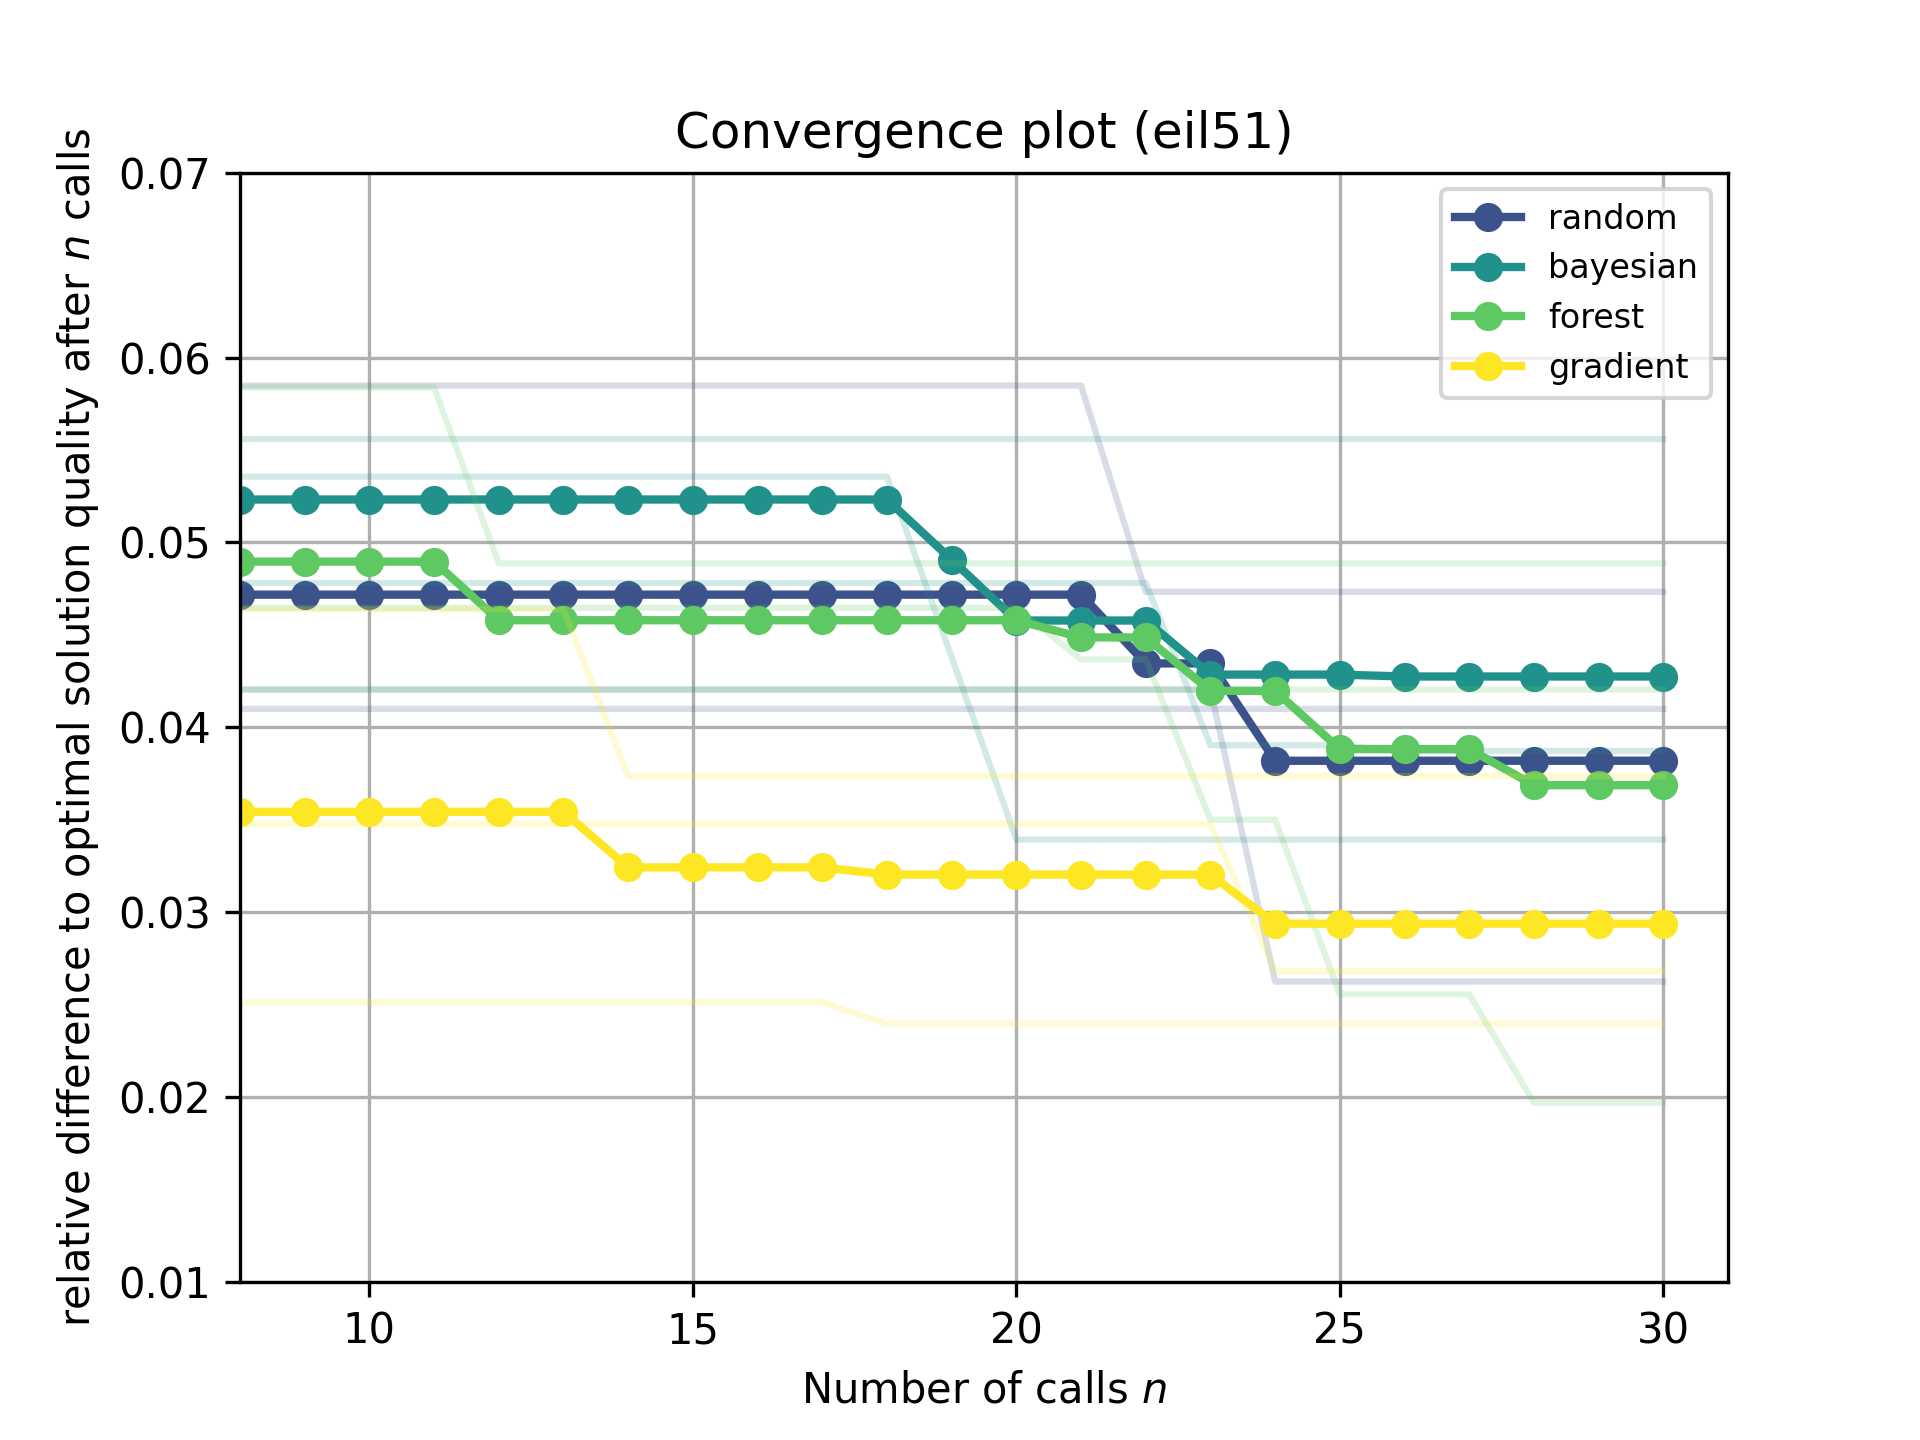
\includegraphics[width=0.75\textwidth]{results/part1/convergence_eil51.png}
	\caption[Convergence plot of \gls{tsp} instance \texttt{eil51}]{Convergence plot of \gls{tsp} instance \texttt{eil51}, comparing four different optimization algorithms.}
	\label{fig:convergence_eil51}
\end{figure}

First, the convergence plots of all five individual instances and their average are discussed. As explained in \cref{chap:an-part1}, these graphs show the minimum of the relative difference to the optimal solution $RPD$ up to each objective function call (\texttt{n\_call}). \cref{fig:convergence_eil51} shows this plot for the \texttt{eil51} \gls{tsp} instance. The bold, yellow line, which shows the average of the three \gls{gbrt} runs, indicates, that this algorithm found the best solution over the course of the 30 objective calls. Except for a single run, where \gls{et} performed admirably, achieving a 2\% difference from the optimal solution, none of the other algorithms were able to come close to the \gls{gbrt}. However, the average convergence behavior of all four algorithms seems to be very similar, with moderate improvements between objective calls 17 and 25. This behavior suggests, that the first 10 sampling calls were sufficient to obtain a decent parameter configuration for the \texttt{eil51} instance. The specific runs (light colored lines) show, that \gls{rs} and \gls{et} fluctuated the most in terms of initial solution quality and improvement over time. Although \gls{gp} produced the worst solutions out of all four algorithms, it still managed to achieve an average solution quality of almost 4\% after the full 30 \texttt{n\_calls}.

\begin{figure}[h]
	\centering
	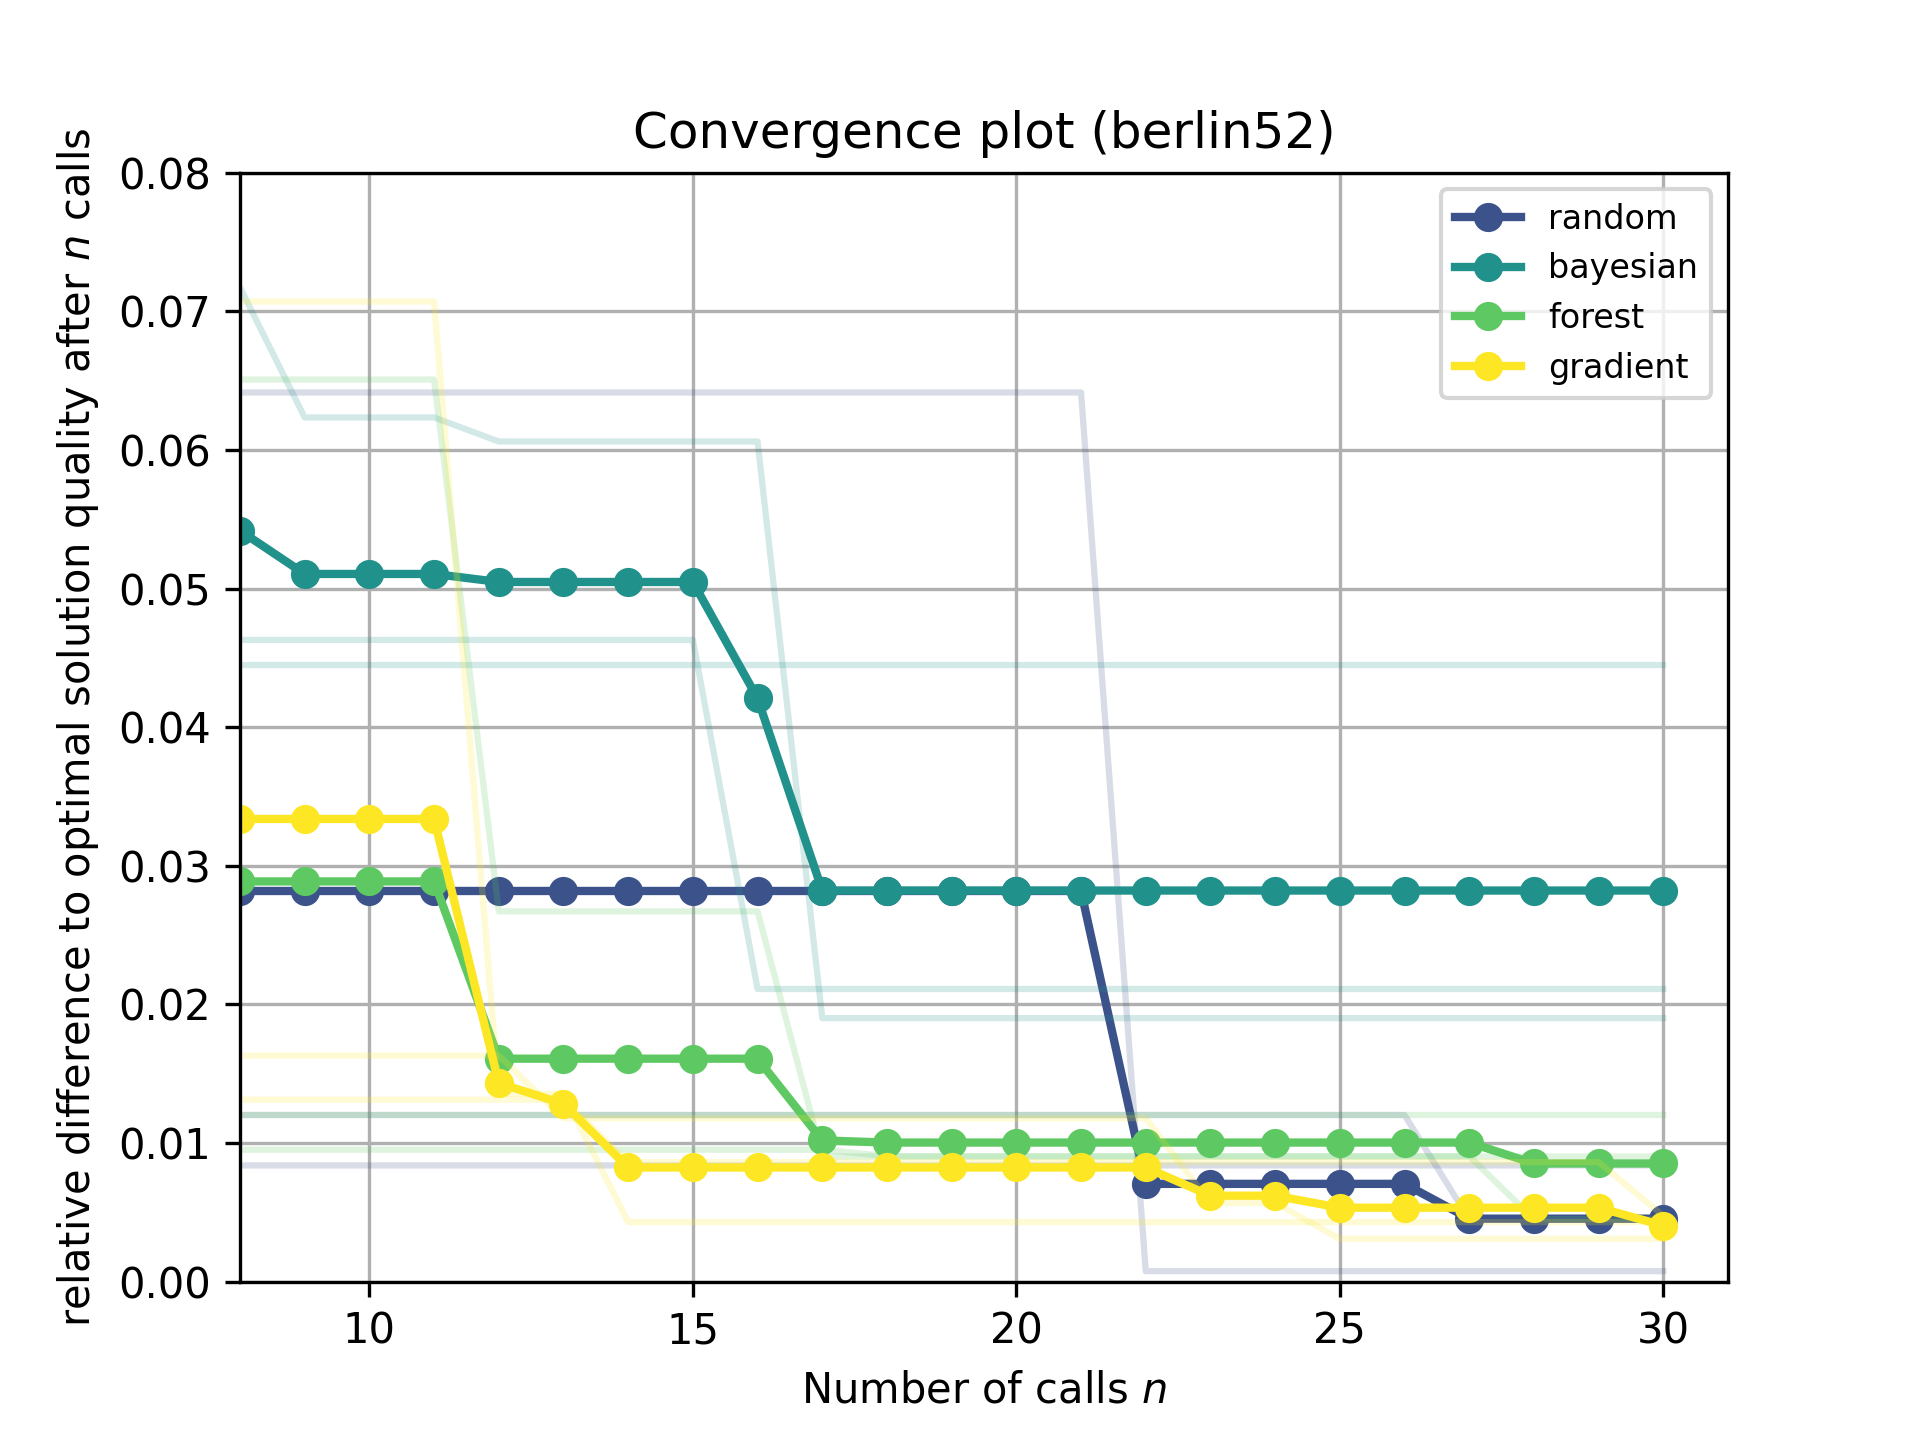
\includegraphics[width=0.75\textwidth]{results/part1/convergence_berlin52.png}
	\caption[Convergence plot of \gls{tsp} instance \texttt{berlin52}]{Convergence plot of \gls{tsp} instance \texttt{berlin52}, comparing four different optimization algorithms.}
	\label{fig:convergence_berlin52}
\end{figure}

The next instance is \texttt{berlin52}, whose convergence plot is shown in \cref{fig:convergence_berlin52}. Here, \gls{gp} continues to be the least well performing \gls{hpo} method, with an average $RPD$ of only about 3\%, with one particular run reaching as low as $4.5\%$. All other methods achieved at least 2\% lower $RPD$ values, with \gls{rs} and \gls{gbrt} having an almost identical final $RPD$ of 0.5\%. 
However, \gls{gp} was able to improve its solution by a significant 2\% over the course of seven additional objective calls, suggesting that the algorithm was quickly making use of the now utilized, underlying model.
Due to the very random nature of \gls{rs}, some other individual runs started with a very high $RPD = 6.5\%$ and then, improved very abruptly after about 21 objective calls. The convergence behavior of \gls{rf} and \gls{gbrt} is quite similar and shows, that both started with a good solution already at about 3\% for the tenth objective call, and then gradually improved up to objective call 17, analogous to \gls{gp}, but with less relative improvement. After that, only small gains in solution quality were achieved.

\begin{figure}[h]
	\centering
	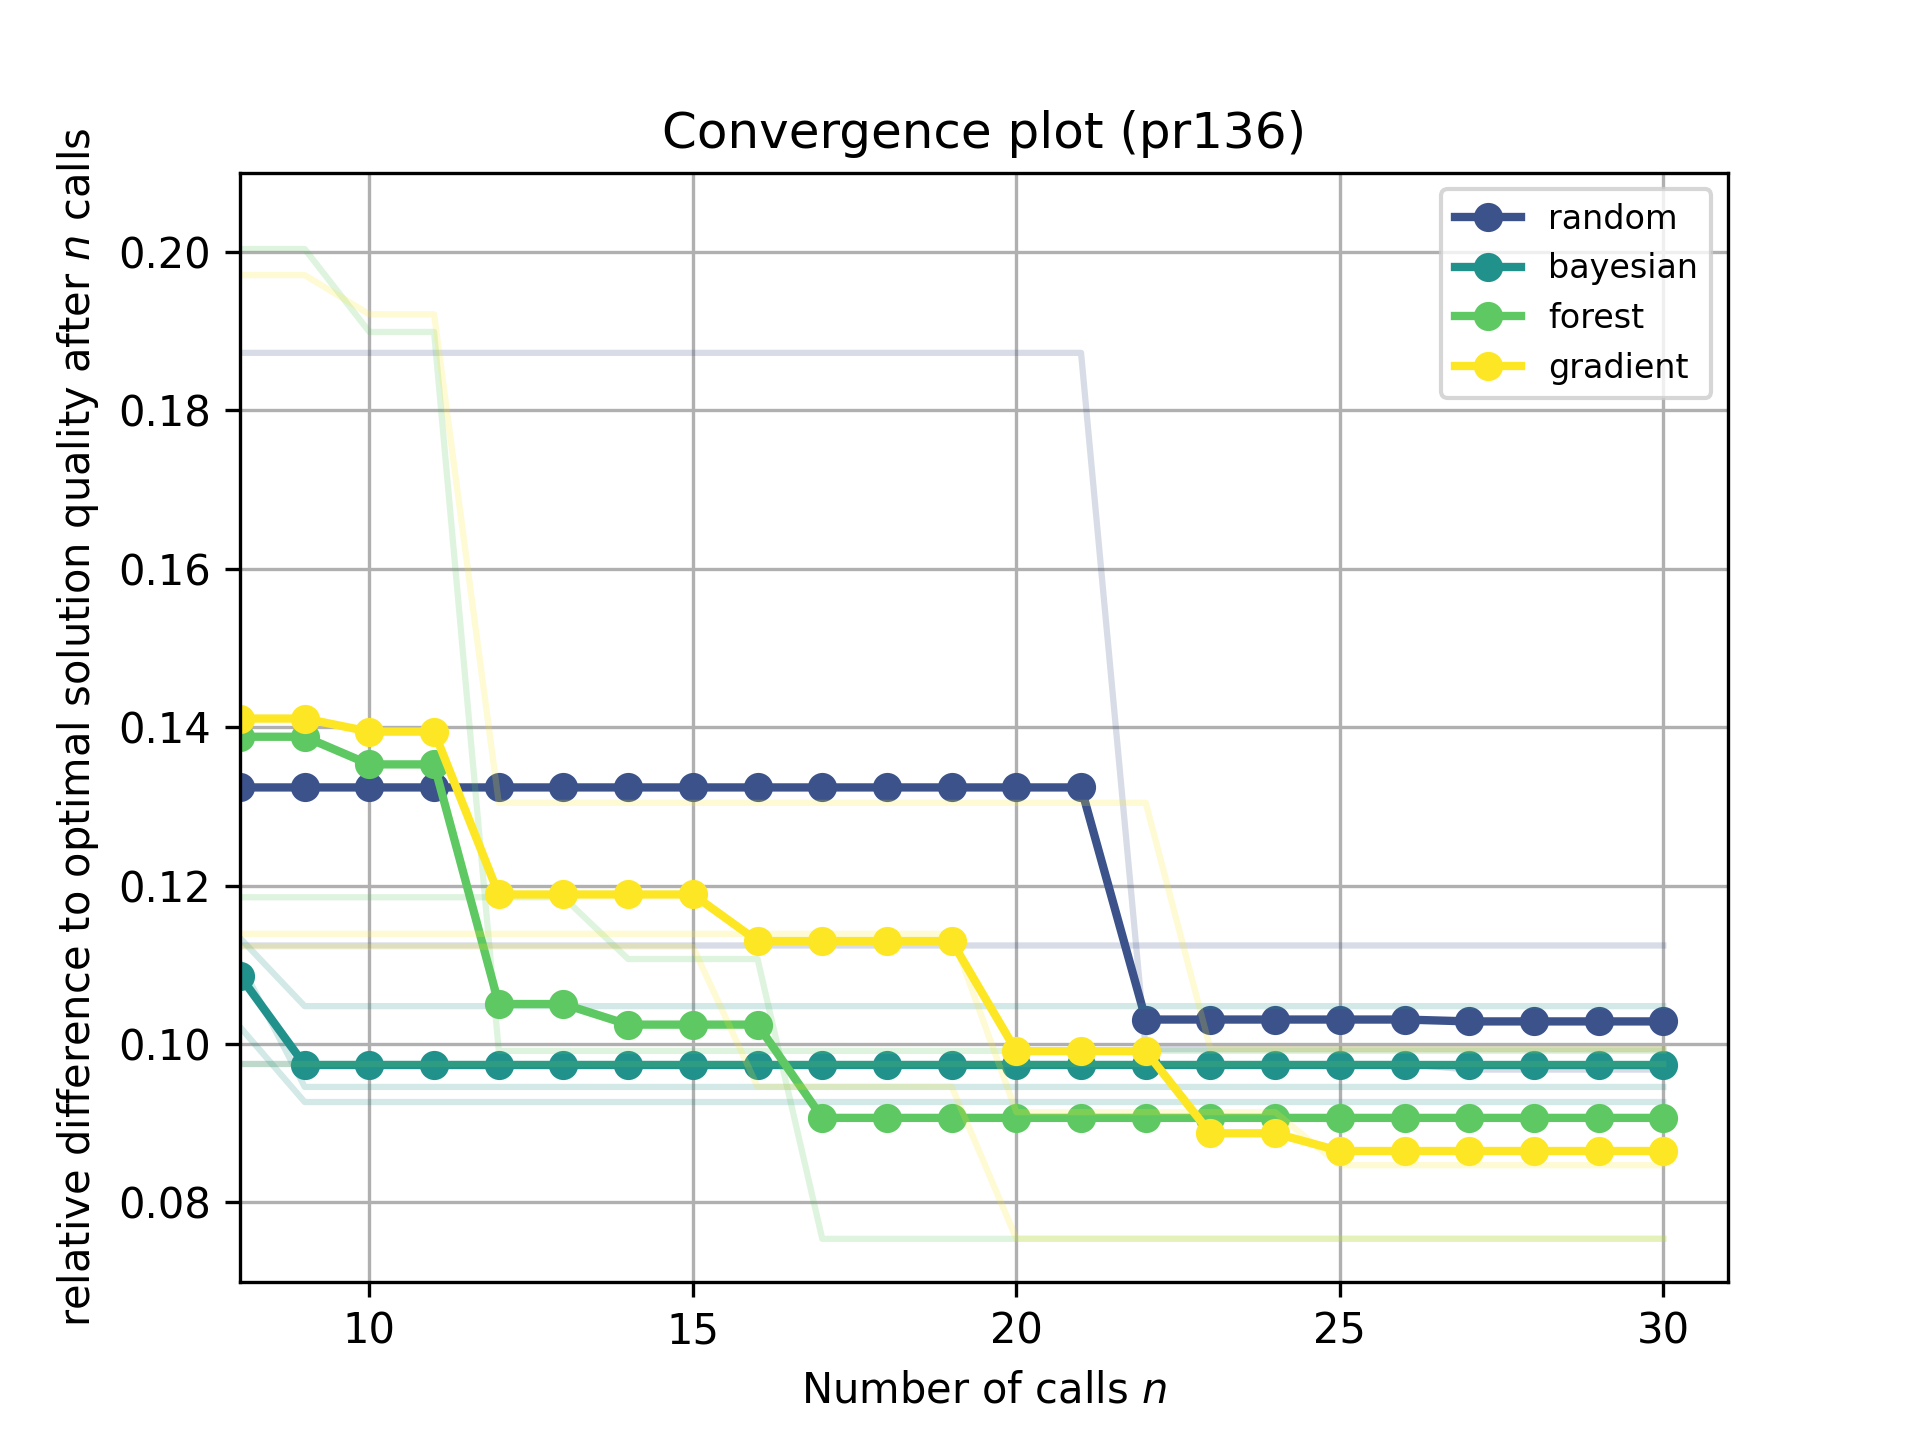
\includegraphics[width=0.75\textwidth]{results/part1/convergence_pr136.png}
	\caption[Convergence plot of \gls{tsp} instance \texttt{pr136}]{Convergence plot of \gls{tsp} instance \texttt{pr136}, comparing four different optimization algorithms.}
	\label{fig:convergence_pr136}
\end{figure}

The \texttt{pr136} \gls{tsp} instance, presented in \cref{fig:convergence_pr136}, continues the trend of \gls{gbrt} performing the best of the four optimization algorithms, albeit with a small lead of less than 0.5\% over the next best method, \gls{et}. Interestingly, \gls{gp} started with a considerably better initial sample at $RPD = 11\%$ after 10 objective calls, which gave it a head start, but also caused the algorithm to stagnate over the course of the remaining 20 calls. This might be due to the fact that Hammersley sampling was chosen only for this particular algorithm, or it could just be another random influence. \gls{et} and \gls{gbrt} gradually improved the most out of the four methods, with steep drops of around 2\% or more by the 23rd objective call. \gls{rs} rarely saw any meaningful improvement after the initial sampling, and the huge drop in average $RPD$ was due only to a single run that remained at a relatively poor value of $RPD = 18.8\%$ up until the 21st \texttt{n\_call}.

\begin{figure}[h]
	\centering
	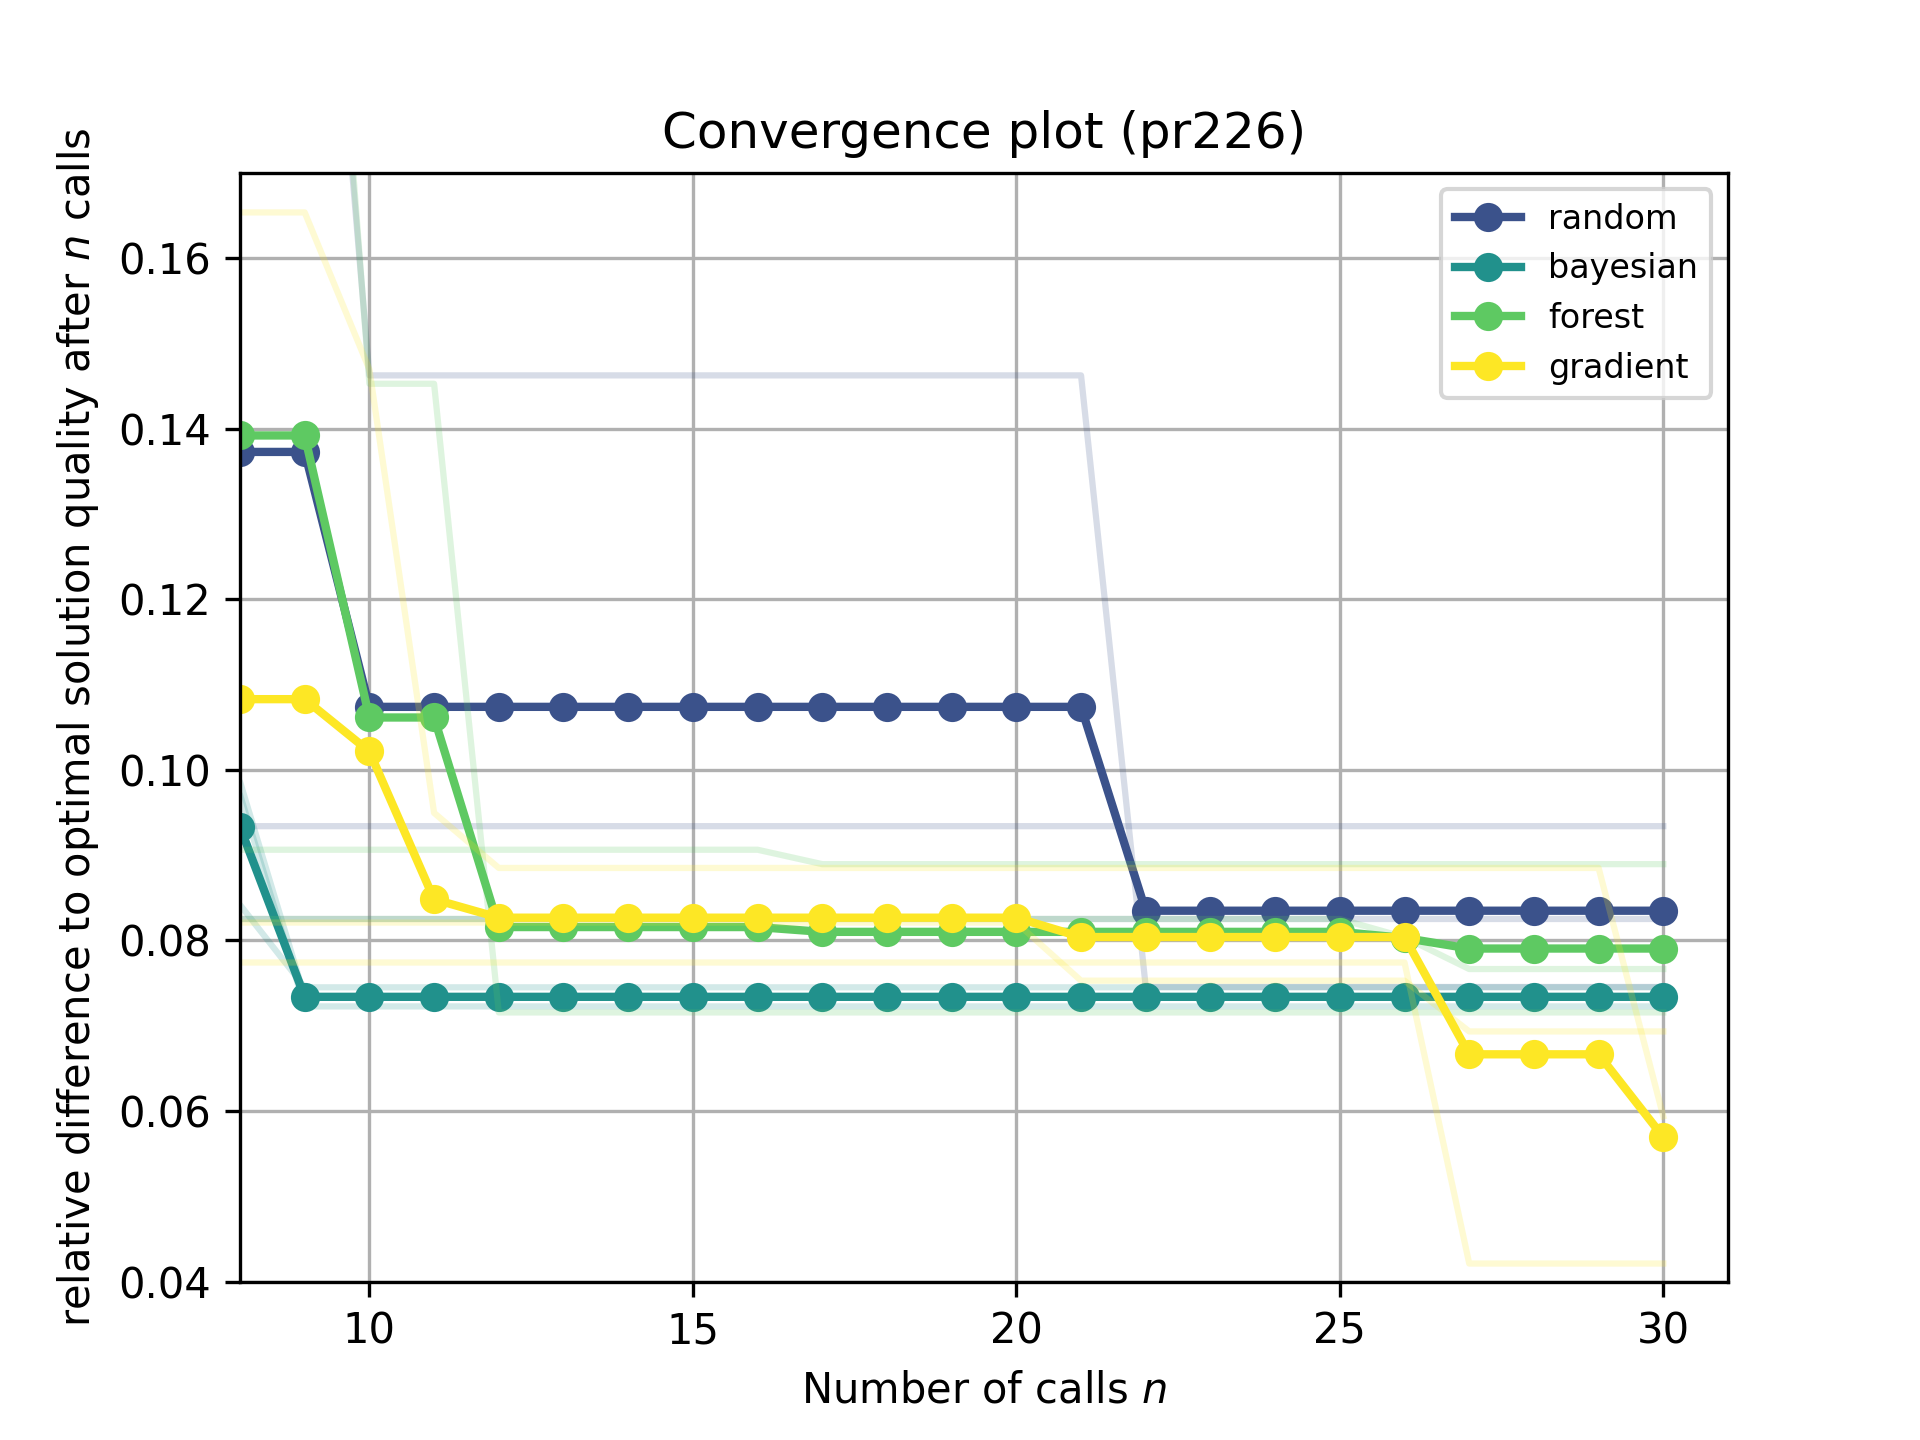
\includegraphics[width=0.75\textwidth]{results/part1/convergence_pr226.png}
	\caption[Convergence plot of \gls{tsp} instance \texttt{pr226}]{Convergence plot of \gls{tsp} instance \texttt{pr226}, comparing four different optimization algorithms.}
	\label{fig:convergence_pr226}
\end{figure}

The convergence plot in \cref{fig:convergence_pr226} for instance \texttt{pr226} again has \gls{rs} as the weakest method, with only small gains of about 2\% on objective call 22, bringing it to the average $RPD$ of the other algorithms. Some other single runs performed even worse. Contrary to the good performance of the other instances, this time \gls{et} starts its model training at 10 objective calls with a $RPD$ value almost the same as \gls{rs}, and only manages to significantly improve its parameters two \texttt{n\_calls} later. It then shows stagnant behavior at $RPD = 8\%$. Only in the last five objective calls \gls{gbrt} showed a similar convergence behavior, improving by more than 2\%, giving it the lead over \gls{gp}. This suggests that with larger instance dimensions and thus potentially more complex solutions, \gls{gbrt} benefits from more objective calls that improve the underlying model.
As with \texttt{pr136}, the initial sample of the Hammersley method gave \gls{gp} a lead in solution quality, but then stagnated after the ninth call and was unable to improve its $RPD$ value of about 7.5\%.

\begin{figure}[h]
	\centering
	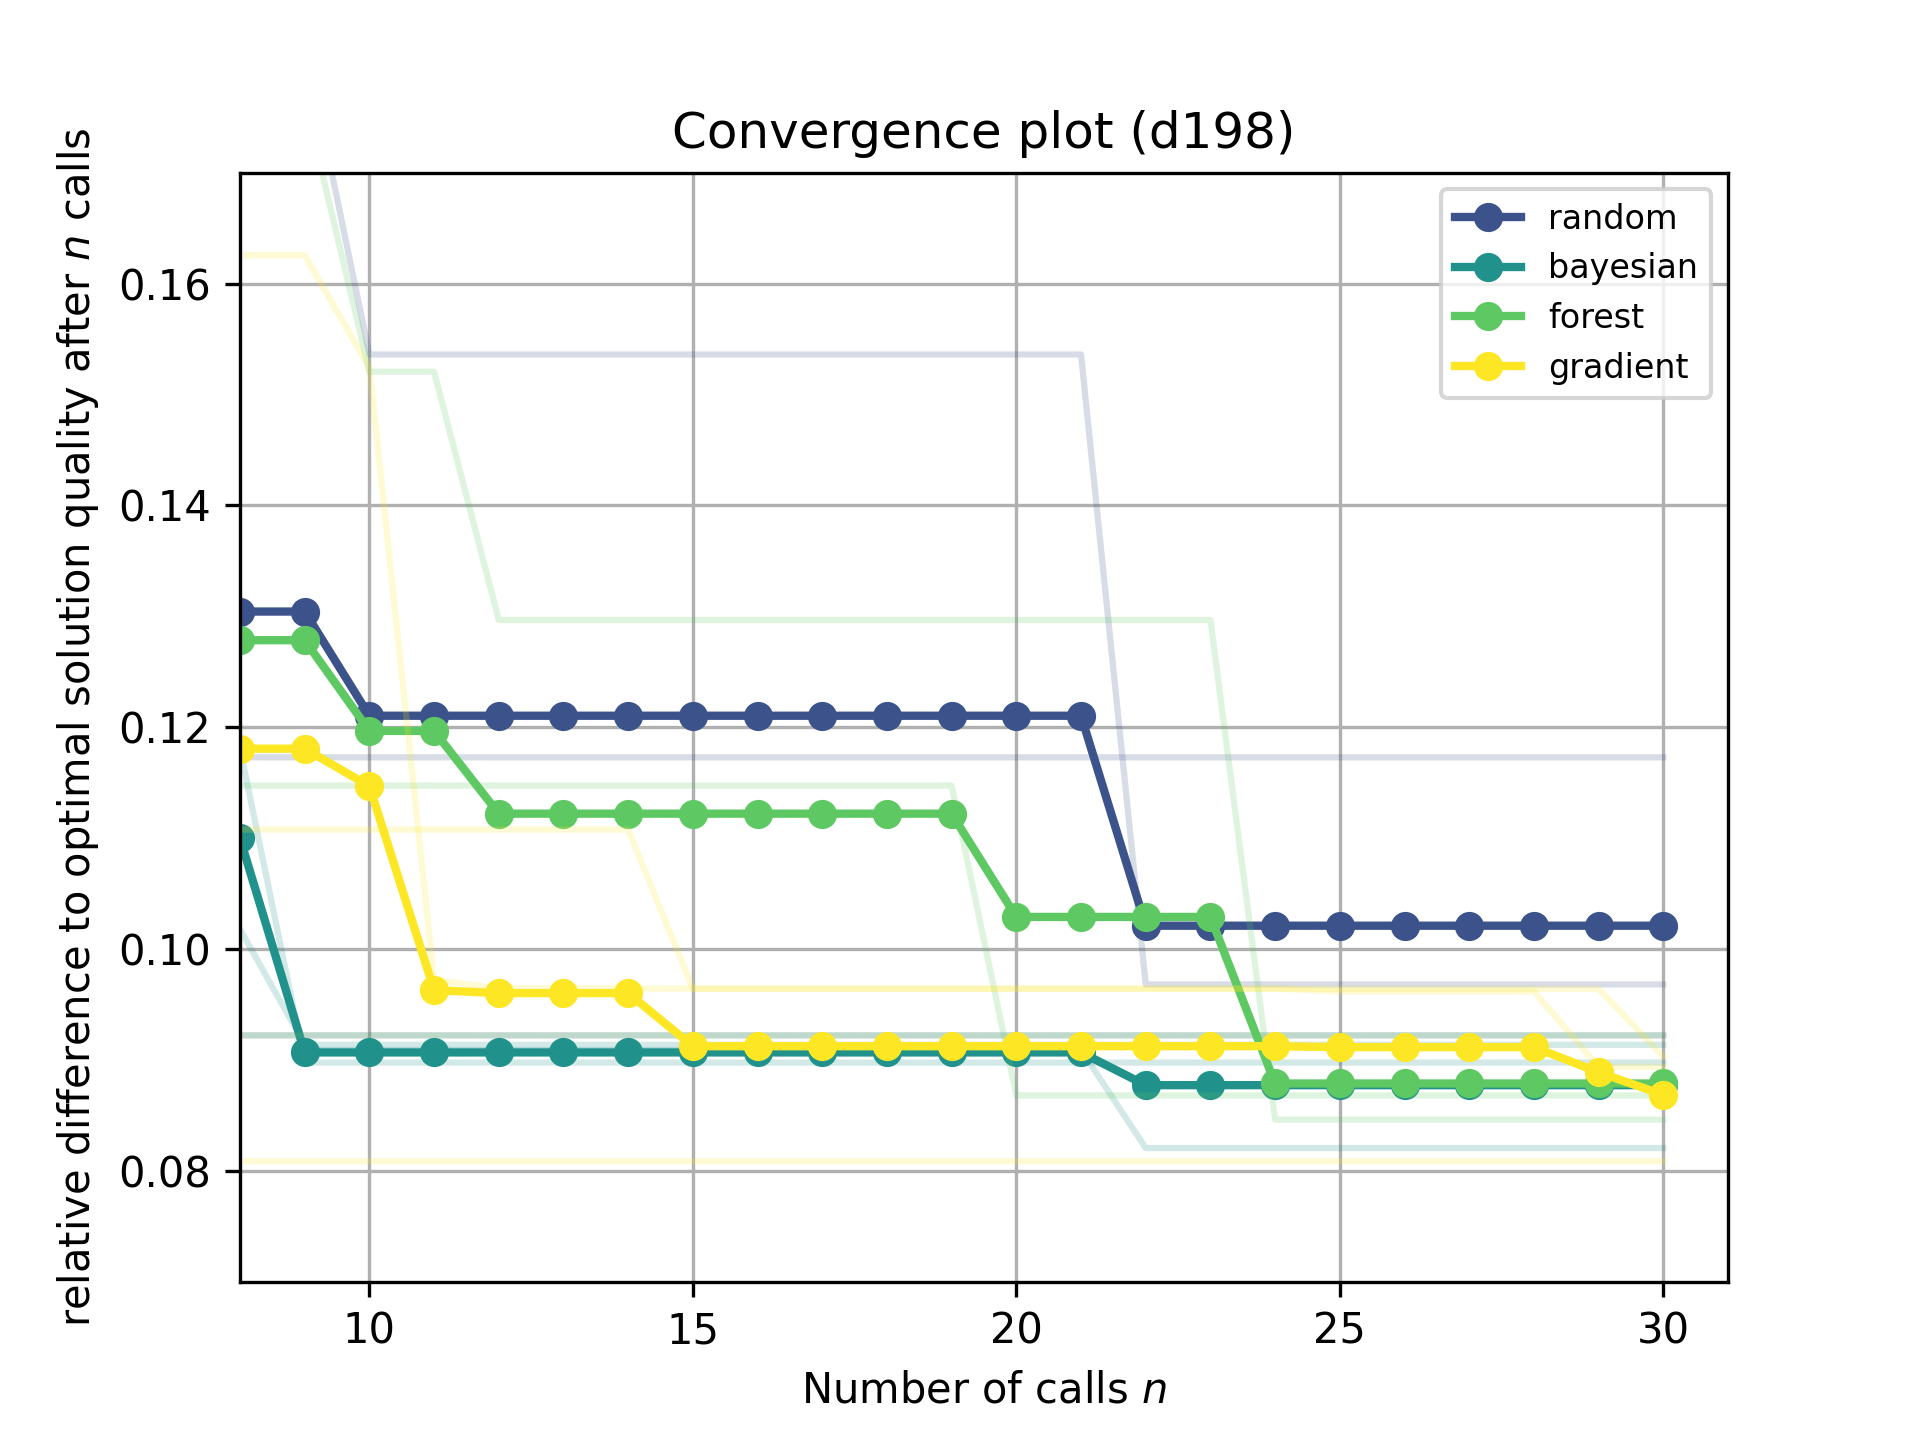
\includegraphics[width=0.75\textwidth]{results/part1/convergence_d198.png}
	\caption[Convergence plot of \gls{tsp} instance \texttt{d198}]{Convergence plot of \gls{tsp} instance \texttt{d198}, comparing four different optimization algorithms.}
	\label{fig:convergence_d198}
\end{figure}

The last \gls{tsp} instance, \texttt{d198}, confirms the observations of the previous instances, but this time all methods except \gls{rs} are within very close proximity to each other after the 24th objective call. Although \gls{gbrt} takes the lead in final relative solution quality with just under 9\%, it is not by much. Together with \gls{gp}, both methods managed to achieve considerable improvements up until the 15th objective call, after which they more or less stagnated. \gls{et} started with a similarly sub-optimal $RPD$ as \gls{rs} at objective call 10, but was able to improve steadily over the next 15 \texttt{n\_calls}. As expected at this point, \gls{rs} only managed to meaningfully improve in one run at objective call 21, still placing its final $RPD$ more than 1\% above the rest of the methods.

\begin{figure}[h]
	\centering
	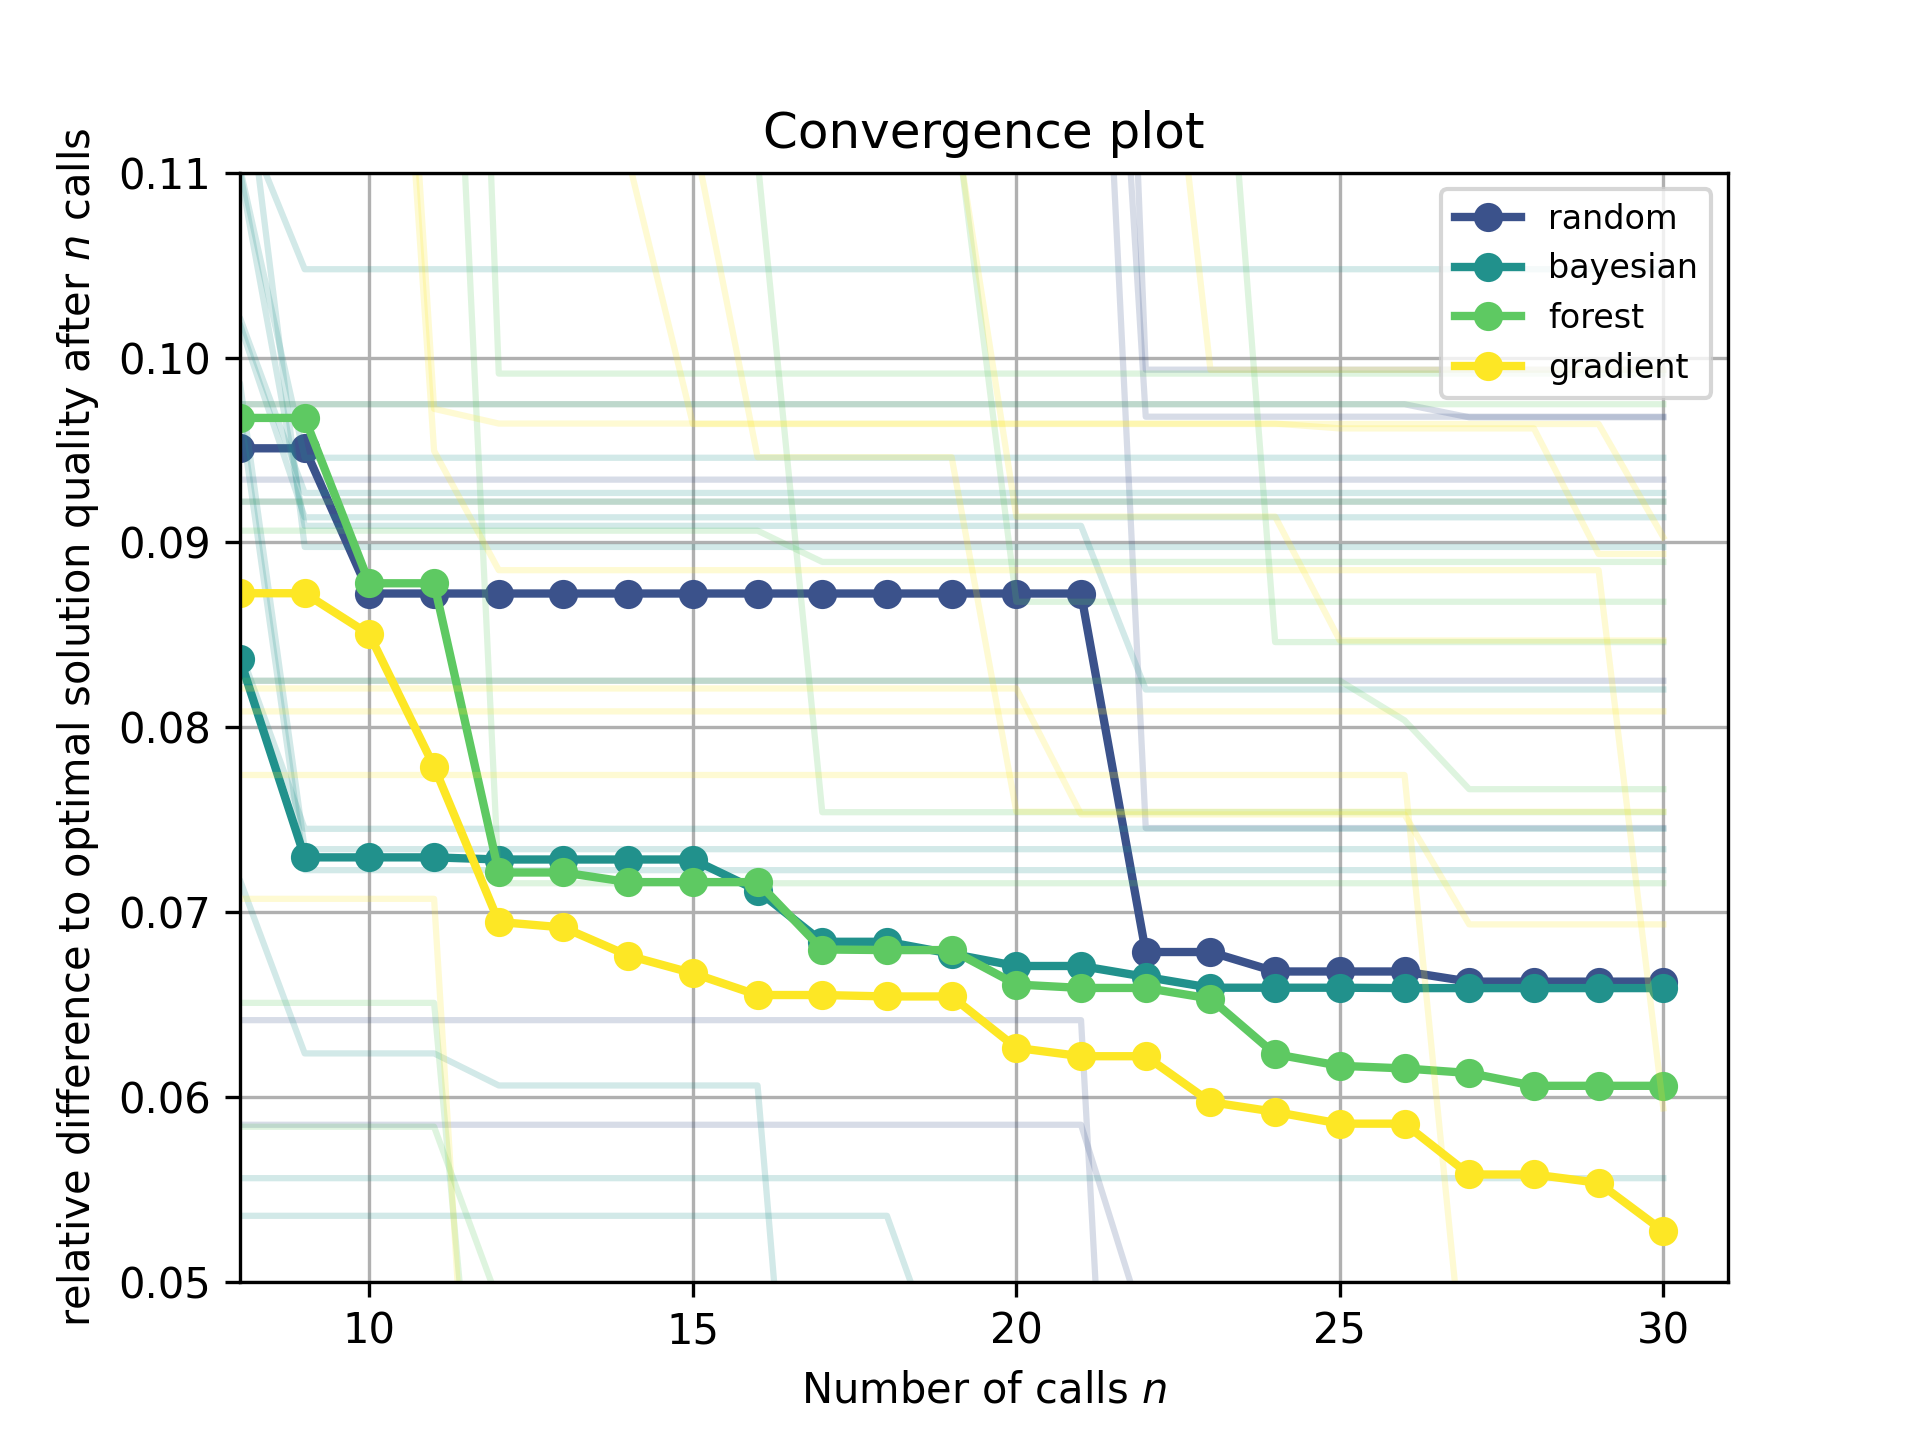
\includegraphics[width=0.75\textwidth]{results/part1/convergence_all.png}
	\caption[Convergence plot of the average over five \gls{tsp} instances]{Convergence plot of the average over five \gls{tsp} instances \texttt{eil51, berlin52, pr136, pr226, d198}, comparing four different optimization algorithms.}
	\label{fig:convergence_all}
\end{figure}

Lastly, the average convergence plot aggregates the runs of all five instances. Since \gls{gbrt} is the best performing method out of all the individual comparisons, its average convergence behavior emphasizes this by giving it a lead in final $RPD$ of about 1.5\% over the next best method, \gls{et}. Both of the show similar convergence behavior over the entire runtime, with large improvements in the first few objective calls, and small, but steady (almost linear) improvements thereafter. The behavior of \gls{gp} is not very different, and is mainly distinguished by its better initial $RPD$ value, which reinforces the proposed relationship with the Hammersley sampling method. After this initial lead, the algorithm almost stagnates, and after the 22nd objective call, it converges to the trajectory of \gls{rs}.

\begin{table}[h]
	\centering
	\caption[The \gls{auc} and $RPD_{min}$ for all optimization runs]{The \gls{auc} and minimum relative solution quality at the last objective call ($RPD_{min}$) of all optimization runs for each method and instance, and for the mean over all instances.}
	\label{tab:part1-stats}
	\begin{tabular}{c !{\vrule width 1pt} c | c !{\vrule width 1pt} c | c !{\vrule width 1pt} c | c }
		~ & \multicolumn{2}{c !{\vrule width 1pt}}{eil51} &  \multicolumn{2}{c !{\vrule width 1pt}}{berlin52} &  \multicolumn{2}{c}{pr136} \\ \hline
		~ & \gls{auc} & $RPD_{min}$ & \gls{auc} & $RPD_{min}$ & \gls{auc} & $RPD_{min}$ \\ \noalign{\hrule height 1pt}
		RS & 0.830 & 0.026 & 0.347 & 0.001  & 2.266 & 0.097 \\ \hline
		GP & 0.900 & 0.034 & 0.650 & 0.019 & 1.850 & 0.093 \\ \hline
		ET & 0.819 & 0.020 & 0.227 & 0.005 & 1.809 & 0.075 \\ \hline
		GBRT & 0.601 & 0.024 & 0.159 & 0.003 & 1.948 & 0.075 \\ 
	\end{tabular}
	\bigskip\\
	\begin{tabular}{c !{\vrule width 1pt} c | c !{\vrule width 1pt} c | c !{\vrule width 1pt} c | c}
		~ & \multicolumn{2}{c !{\vrule width 1pt}}{pr226} & \multicolumn{2}{c !{\vrule width 1pt}}{d198} & \multicolumn{2}{c}{mean}\\ \hline
		~ & \gls{auc} & $RPD_{min}$ & \gls{auc} & $RPD_{min}$ & \gls{auc} & $RPD_{min}$ \\ \noalign{\hrule height 1pt}
		RS &  1.837 & 0.075 & 2.139 & 0.092 & 1.484 & 0.058\\ \hline
		GP & 1.394 & 0.072 & 1.698 & 0.082 & 1.298 & 0.060\\ \hline
		ET & 1.547 & 0.072 & 1.940 & 0.085 & 1.268 & 0.051\\ \hline
		GBRT & 1.497 & 0.042 & 1.745 & 0.081 & 1.190 & 0.045\\ 
	\end{tabular}
\end{table}

Regarding the visually observable convergence behavior of the four optimization methods, we can also look at the \glsfirst{auc} of the plots and the minimum/best relative solution quality obtained, i.e. the $RPD$ value at $\texttt{n\_call} = 30$, hereafter called $RPD_{min}$. This data is presented in \cref{tab:part1-stats} for all five instances, their mean, and is made up of all available optimizer runs.
In this context, a low \gls{auc} value would indicate that the optimization algorithm found a well-performing parameter set, and therefore a low $RPD$, in a short time, i.e., few objective calls. However, the comparatively lowest \gls{auc} does not necessarily mean that it also found the lowest $RPD_{min}$ value among all algorithms. Thus, both values are discussed for each instance to determine how fast each algorithm converged to its best solution. For the \texttt{eil51} \gls{tsp} instance, \gls{gbrt} has by far the lowest \gls{auc} of 0.601. Paired with the second best $RPD_{min} = 2.4\%$, this method continues its favorable performance from the convergence plots. With a 0.4\% improvement in $RPD_{min}$ over \gls{gbrt}, \gls{et} was the second fastest to convergence to this final solution. \gls{gp} delivered the worst performance in this instance.

The \texttt{berlin52} instance implies a similar behavior, with \gls{gbrt} leading in convergence speed via the lowest \gls{auc}. However, as discussed in the corresponding convergence plot, \gls{rs} managed to find the best solution out of the four methods, with $RPD_{min} = 0.1\%$, outperforming \gls{gbrt} by 0.2\%. Again, \gls{gp} shows the worst performance, this time with an \gls{auc} of $0.650$, almost twice as high as its direct competitor \gls{rs} with $0.347$. \gls{et} is again the second fastest converging algorithm after \gls{gbrt}, with an almost equally good $RPD_{min} = 0.5\%$.

The results for \texttt{pr136} show an equal best $RPD_{min} = 7.5\%$ for \gls{gbrt} and \gls{et}, and an almost equal \gls{auc} for \gls{gp} and \gls{et}. Therefore, in this instance, \gls{et} outperforms \gls{gbrt} as the best converging algorithm. Interestingly, even \gls{gp} achieves a better \gls{auc} of $1.850$ than \gls{gbrt}, albeit with a worse minimum relative solution quality, which is more in line with \gls{rs}.

\texttt{pr226}, the largest \gls{tsp} instance out of the five tested in this part of the experimentation discussion, continues the improvement of \gls{gp} in terms of \gls{auc}, resulting in the best value out of all four algorithms, with a solid 7\% difference compared to the next best algorithm, \gls{gbrt}, which itself, was able to achieve the best $RPD_{min}$ at 4.2\%. \gls{rs} continues to perform worse as the instance dimension increases, which could be an opposite trend for the convergence speed of \gls{gp}.

The last \gls{tsp} instance, \texttt{d198}, confirms this implication, resulting in \gls{gp} again being the best algorithm in terms of \gls{auc}, and the second best in terms of $RPD_{min}$ at 8.2\%. This suggests, that this algorithm could benefit from larger, more complex instances, perhaps even from stronger clustering, as the latter two instances were categorized. \gls{gbrt} achieved the best $RPD_{min}$ value at 8.1\% and the second best \gls{auc}, which is only 2.7\% higher than the value of \gls{gp}. In this instance, the performance of \gls{et} was comparatively underwhelming, being closer to the \gls{auc} value of \gls{rs} than to the other two methods.

Finally, the mean results confirms, that \gls{gbrt} was the algorithm that converged the fastest ($\gls{auc} = 1.19$) to the best performing parameter set ($RPD_{min} = 4.5\%$). Even in later, higher dimensional  instances, it performed at least the second best or better, implying good search consistency across the parameter space. \gls{et} obtained better solutions at an earlier time for the three smaller instances, resulting in lower averages compared to \gls{gp}, which showed the opposite trend, improving with higher problem dimension.

\begin{figure}[h]
	\centering
	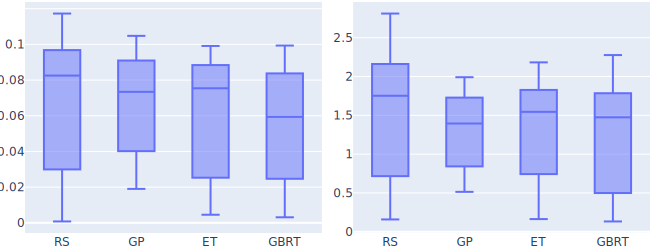
\includegraphics[width=\textwidth]{results/part1/convergence_stats_boxplot.svg}
\captionsetup[subfigure]
{skip=-8pt}
		\hfill
		\subcaptionbox{Relative difference to optimal solution quality at last the objective call ($RPD_{min}$) for all runs and instances.\label{fig:convergence_stats_boxplot_rpd_min}}[.45\linewidth]{\hfill}
		\hfill
		\subcaptionbox{\Glsfirst{auc} of solution quality convergence graph.\label{fig:convergence_stats_boxplot_auc}}[.45\linewidth]{\hfill}

	\caption[Statistical box plots illustrating convergence plots]{Statistical box plots illustrating the data of all five individual convergence plots and their individual runs.}
\label{fig:convergence_stats_boxplots}
\end{figure}

\Cref{fig:convergence_stats_boxplots} shows statistical box plots for both of the metrics from the table over all runs and not grouped by instance. This visualization is also used to evaluate the consistency across all four optimization methods, which was previously only implied by their average or best-case performance. However, this is not normalized by instance, so the absolute values and differences, as with the mean from the previous table, might not be as expressive. Nevertheless, since all four algorithms are affected by this bias, qualitative statements are still possible.

The dispersion of $RPD_{min}$ in \cref{fig:convergence_stats_boxplot_rpd_min} implies that \gls{gp} reached its solution most consistently at around its median of 7.5\%, but also never reached the same minimum as the other three algorithms. \gls{rs}, on the other hand, was the most unreliable method, with its maximum and minimum being far of from the upper and lower quartiles, respectively. It also has the highest median at about 8\%. \gls{gbrt} and \gls{et} share similarities in their \gls{iqr} and minimum/maximum values, with \gls{gbrt} having a slightly smaller dispersion. However, they differ tremendously in their median, with \gls{et} having a value almost 2\% higher than \gls{gbrt}, which means that although both their solution consistency is not ideal, \gls{gbrt} still obtained the best final solution out of all algorithms.

The box plots for the \gls{auc} (\cref{fig:convergence_stats_boxplot_auc}) show similar consistency behavior. \gls{gp} is again the most reliable algorithm when it comes to converging to its final solution, but again it cannot provide the same best-case performance (minimums) as the other three algorithms. Howeer, its median is the lowest, with \gls{gbrt} having the second lowest value, but also a significantly higher \gls{iqr} than \gls{gp}. Lastly, \gls{rs} shows the most inconsistent behavior with the highest median. 

\subsection{Statistical Tests}

To validate all of the above results, two statistical tests were also performed on the optimization data. The first test was the Kruskal–Wallis H test, explained in section \cref{chap:kruskal}, with each of the four optimization algorithms as a sample group, and separated by the five instances used. The results for each instance are shown in \cref{tab:kruskal-test}. A common significance level of 0.05 was chosen to reject the null hypothesis. The data from the table shows, that for each of the five instances, we can definitely reject the null hypothesis by looking at the $p$-values, thus suggesting that the four optimization algorithms show a significantly different convergence behavior from each other. 

\begin{table}[h]
	\centering
	\caption[Results of the Kruskal–Wallis H test for all optimization run data of the first part]{Results of the Kruskal–Wallis H test for all optimization run data of the first part, with each of the four optimization algorithms as a sample group, separated by \gls{tsp} instance.}
	\label{tab:kruskal-test}
	\begin{tabular}{l|l|l|l|l|l}
		~ & eil51 & berlin52 & pr136 & pr226 & d198 \\ \hline
		statistic & 47.893 &	46.960&	29.898	&57.998	&46.514 \\
		$p$-value & \num{2.244e-10} & \num{3.544e-10} &\num{1.450e-6} & \num{1.574e-12} & \num{4.410e-10} \\
	\end{tabular}
\end{table}
\texttt{}

A post-hoc Conover–Iman test was then performed to gain more insight into which specific pairs of optimization algorithms differ and how. As explained in \cref{chap:conover}, a one-sided test was used, resulting in two tables - one for the statistic value (\cref{tab:conover-t}) and one for the $p$-value (\cref{tab:conover-p}). Note that this table format was preferred over a symmetric matrix for each problem instance, with the columns and rows containing all five methods each. As presented here, redundant information can be excluded by directly pairing the algorithms, resulting in $\binom{4}{2} = 6$ pairs (columns) for each \gls{tsp} instance (rows). 

Starting with the $p$-value to reject the null hypothesis, we can then look at the statistic value, more specifically at the sign, to formulate the alternative hypothesis, i.e. to infer how the distribution of the convergence behavior for the algorithms differ. A positive value implies that in this particular pairwise comparison (X vs. Y), the first stated algorithm (X) has a distribution that is significantly above the others, suggesting that either the convergence speed, the solutions obtained, or both, are also worse than the second one (Y). Furthermore, in both tables the cells are marked green, whenever the $p$-value is lower than 0.05 (the significance level) and the null hypothesis can be rejected for that combination of \gls{tsp} instance and optimization method pairing.

\begin{table}[h]
	\centering
	\caption[The $p$-value of the Conover–Iman test for all optimization run data of the first part]{The $p$-value of the Conover–Iman test for all optimization run data of the first part, with each of the four optimization algorithms as a sample group, separated by \gls{tsp} instance. The cells are marked green, whenever the $p$-value is lower than the significance level of $0.05$.}
	\label{tab:conover-p}
	
	\begin{adjustbox}{width=1\textwidth}
		\begin{tabular}{ l | l | l | l | l | l | l}
			TSP & \gls{rs} vs. \gls{gp} & \gls{rs} vs. \gls{et} & \gls{rs} vs. \gls{gbrt} & \gls{gp} vs. \gls{et} & \gls{gp} vs. \gls{gbrt} & \gls{et} vs. \gls{gbrt} \\ \hline
			eil51 & \num{0.626022837} & \num{1} & \cellcolor{green!25} \num{1,3613E-11} & \cellcolor{green!25} \num{0,045498418} &  \cellcolor{green!25} \num{9,87937E-15} &\cellcolor{green!25}  \num{1,71033E-09} \\ \hline
			berlin52 & \cellcolor{green!25} \num{6,31757E-10} & \num{1} & \num{0,055983678} & \cellcolor{green!25} \num{4,84375E-08} & \cellcolor{green!25} \num{5,09448E-15} & \cellcolor{green!25} \num{0,002694824} \\ \hline
			pr136 & \cellcolor{green!25} \num{4,40687E-06} &\cellcolor{green!25}  \num{1,47269E-07} & \cellcolor{green!25} \num{1,49122E-04} & \num{1} & \num{1} & \num{0,524644367} \\ \hline
			pr226 & \cellcolor{green!25} \num{1,07734E-22} & \cellcolor{green!25} \num{1,85077E-10} & \cellcolor{green!25} \num{1,83947E-11} & \cellcolor{green!25} \num{2,22893E-08} & \cellcolor{green!25} \num{2,06853E-07} & \num{1} \\ \hline
			d198 & \cellcolor{green!25} \num{4,0384E-15} & \cellcolor{green!25} \num{0,001090407} & \cellcolor{green!25} \num{2,6556E-07} & \cellcolor{green!25} \num{1,20061E-07} & \cellcolor{green!25}  \num{0,000563675} & \num{0,210301266} \\
		\end{tabular}
	\end{adjustbox}
\end{table}

\begin{table}[h]
	\centering
	\caption[The $p$-value of the Conover–Iman test for all optimization run data of the first part]{The statistical value of the Conover–Iman test for all optimization run data of the first part, with each of the four optimization algorithms as a sample group, separated by \gls{tsp} instance. The cells are marked green, whenever the $p$-value is lower than the significance level of $0.05$.}
	\label{tab:conover-t}
	
	\begin{adjustbox}{width=1\textwidth}
	\begin{tabular}{ l | l | l | l | l | l | l}
		TSP & \gls{rs} vs. \gls{gp} & \gls{rs} vs. \gls{et} & \gls{rs} vs. \gls{gbrt} & \gls{gp} vs. \gls{et} & \gls{gp} vs. \gls{gbrt} & \gls{et} vs. \gls{gbrt} \\ \hline
		eil51 & \num{-1,643854208} & \num{1,099460932} & \cellcolor{green!25} \num{8,358037955} & \cellcolor{green!25} \num{2,74331514} & \cellcolor{green!25} \num{10,00189216} & \cellcolor{green!25} \num{7,258577024} \\ \hline
		berlin52 & \cellcolor{green!25} \num{-7,486334021} & \num{-1,00169258} & \num{2,667665503} & \cellcolor{green!25} \num{6,484641441} & \cellcolor{green!25} \num{10,15399952} & \cellcolor{green!25} \num{3,669358084} \\ \hline
		pr136 & \cellcolor{green!25} \num{5,39986544} & \cellcolor{green!25} \num{6,222702079} & \cellcolor{green!25} \num{4,491316652} & \num{0,822836638} & \num{-0,908548788} & \num{-1,731385427} \\ \hline
    	pr226 & \cellcolor{green!25} \num{14,43190942} & \cellcolor{green!25} \num{7,765991183} & \cellcolor{green!25} \num{8,289835445} & \cellcolor{green!25} \num{-6,665918233} & \cellcolor{green!25} \num{-6,142073971} & \num{0,523844262} \\ \hline
    	d198 & \cellcolor{green!25} \num{10,20744357} & \cellcolor{green!25} \num{3,936409009} & \cellcolor{green!25} \num{6,082589453} & \cellcolor{green!25} \num{-6,271034565} & \cellcolor{green!25} \num{-4,124854122} & \num{2,146180444} \\ 
	\end{tabular}
	\end{adjustbox}
\end{table}

The data from both tables show, that the distribution of the \gls{gbrt} method is below all other algorithms for the \texttt{eil51} instance, although the null hypothesis in the pairing with \gls{et} was only slightly below the significance level. Furthermore, the distribution of \gls{et} was also below that of \gls{gp}, confirming the visual inference from the convergence plot. 
In the data for the \texttt{berlin52} instance, \gls{gbrt} is below \gls{gp} and \gls{et}, but interestingly, fails to reject the null hypothesis when compared to \gls{rs}, confirming the unrepresentatively good performance of this algorithm for this instance. Also, the convergence distribution of \gls{gp} is above all other three algorithms by comparison, which is also shown in \cref{fig:convergence_berlin52}.
For the next three instances, \texttt{pr136, pr226,} and \texttt{d198}, the distribution for \gls{rs} lies above all other three algorithms, verifying the underwhelming performance described in previous discussion. For the two latter instances, we can also determine that the convergence behavior of \gls{gp} is above the distribution of both \gls{et} and \gls{gbrt}.

In summary, \gls{rs} could only establish itself as having a favorable distribution only once, \gls{et} managed to have a lower convergence behavior five times, \gls{gp} could undercut in its direct pairing seven times, and \gls{gbrt} was the optimization algorithm that fell below its comparison distribution the most with 10 times. All of this confirms the favorable position of \gls{gbrt}, but also strengthens the case for \gls{gp} over \gls{et}.

\subsection{Conclusion}

As expected, \glsfirst{rs} proved to be the worst performing algorithm under these test conditions. Although each of the other three methods was able to reliably outperform its solutions, usually with fewer objective calls, it still produced satisfactory solutions that differed from the rest by only a few percent. Therefore, its aforementioned position as a \enquote{baseline} \gls{hpo} method is more than justified.

The \glsfirst{gbrt} algorithm shows the fastest convergence with the best solution quality, while providing the second most robust results. Therefore, it is used to perform the second part of the testing procedure. Another advantage, besides its good performance, is its ability to provide a trained machine learning model from which the parameter importance and other qualitative statements about its prediction can be derived.

However, the theoretical second choice is not so clear, since both \glsfirst{gp} and \glsfirst{et}, performed very well in certain instances. As suggested in some earlier discussions, \gls{et} seems to perform its best on \gls{tsp} instances with less than 100 city nodes, while \gls{gp} improves its convergence and solutions significantly on \gls{tsp} instances with dimensions above 150. Another factor may be the city placement characteristic established in \cref{chap:problem-choice}. However, confirming this possible relationship would require a different experimental setup, whereas the data from this first part would not be sufficient. Therefore, both of these algorithms should be considered as potential candidates for future tests, especially with varying problem dimensions and complexity.


\section{Part II - Choosing the Parameter Sets}
\label{chap:part2}

\subsection{Robustness of Parameter Values}

\subsection{Correspondence with Problem Instances}

\subsection{Parameter Importance}


\section{Part III - Evaluating the Parameter Sets}
